\newpage
\section{Admin-Specific Features}

University Management system contains three main users that have access to this software, administrators, students, and faculty. Administrators are the users who have the highest level of privileges between all users with access to this software. They allow for the addition and deletion of specific features and users in the university management system.


\subsection{Subject Management}

The subject management tab allows administrators to add a specific subject to the University of Guelph. These subjects range between all the different departments for all the different colleges. Only administrators can make these changes as they have the required access and privileges to do so. In \autoref{fig:example5}, it showcases the subject management tab, in this tab administrators can either add a subject or delete a subject. First, adding a subject by entering their Subject Code and Subject Name, and deleting a subject by selecting the specific subject and clicking the red delete button. The removal of subjects comes from changes in the University Administration, low enrolment of students in a course, or changes in the overall program. \\

The process of adding and deleting a subject goes as follows.
\begin{enumerate}
    \item Administrator enters the Subject Code and the Subject Name
    \item Administrator press the Add Subject button
    \item Administrator review the table to ensure that the require course has been added
    \item Administrator can delete a course by selecting the targeted course resulting in a highlight. Then press the Delete Subject button.
    \item Data entries are saved in the integrated excel file.
\end{enumerate}

\textbf{Note:} The subject management tab is available for users such as faculty and students, however they do not have the ability to remove or add courses. They must have administrator login credentials for complete those tasks. 

\begin{figure}[h!]
    \centering
    \centering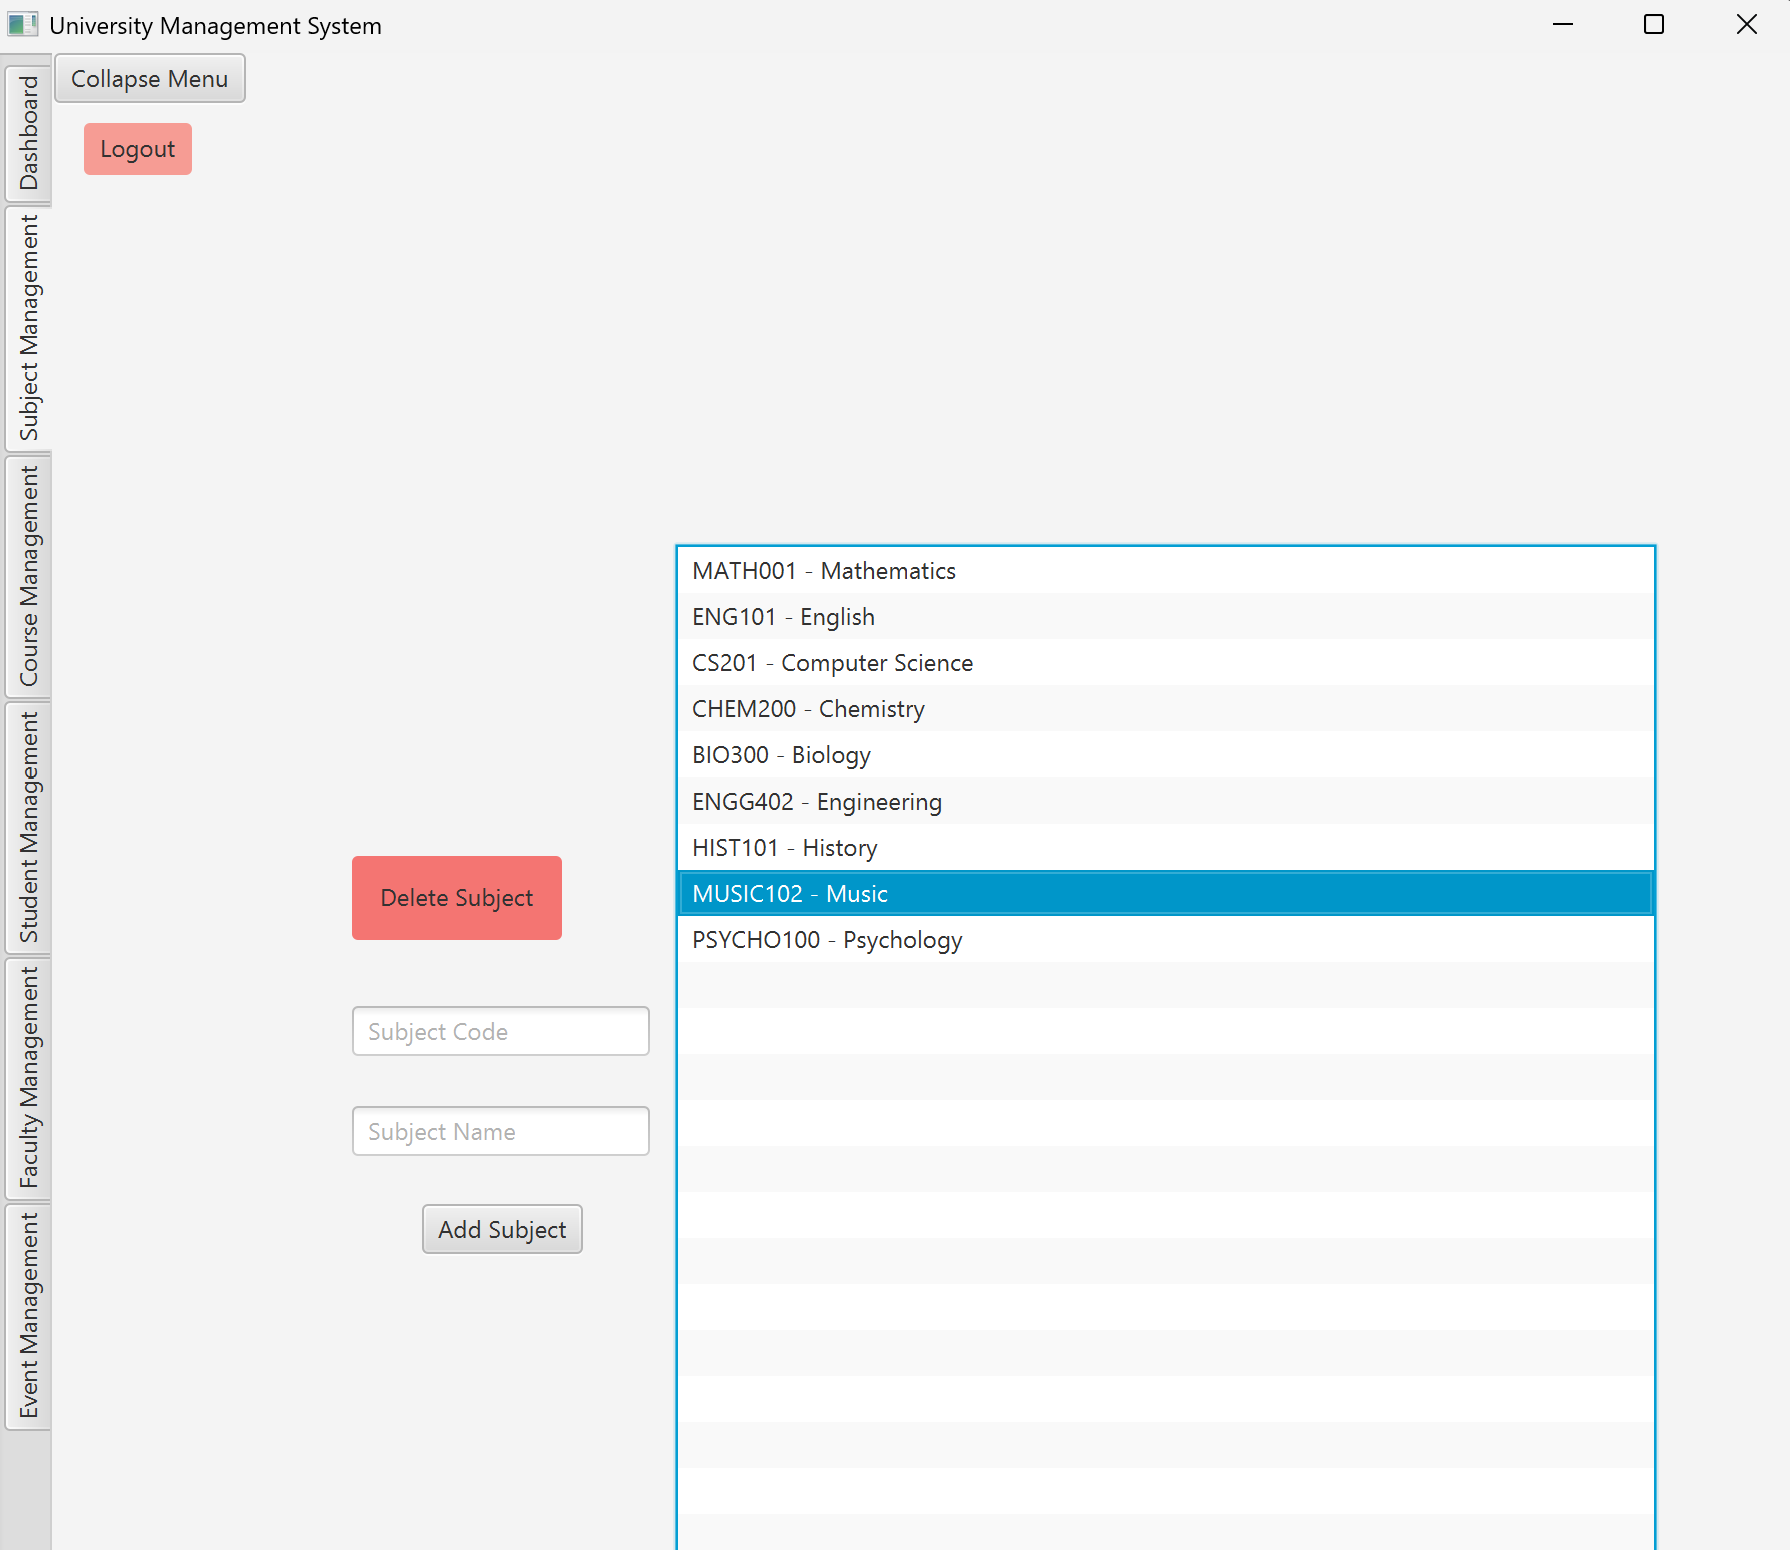
\includegraphics[width=0.7\linewidth]{figures/Subject_Management.png}
        \caption{Administrator Login - Subject Management Tab}
        \label{fig:example5} 
\end{figure}

\newpage
\subsection{Student Management}

The Student Management tab for administrators provides the administrator with the privilege of adding students to the University Management System, refer to \autoref{fig:example6} The procedure to add students is achieved by following the specific steps.

\begin{enumerate}
    \item Administrate clicks the input name field
    \item Administrator enters the student's name, email Student ID, and address, by clicking enter each time to store the information within the system and excel data archival file.
\end{enumerate}

\begin{figure}[h!]
    \centering
        \centering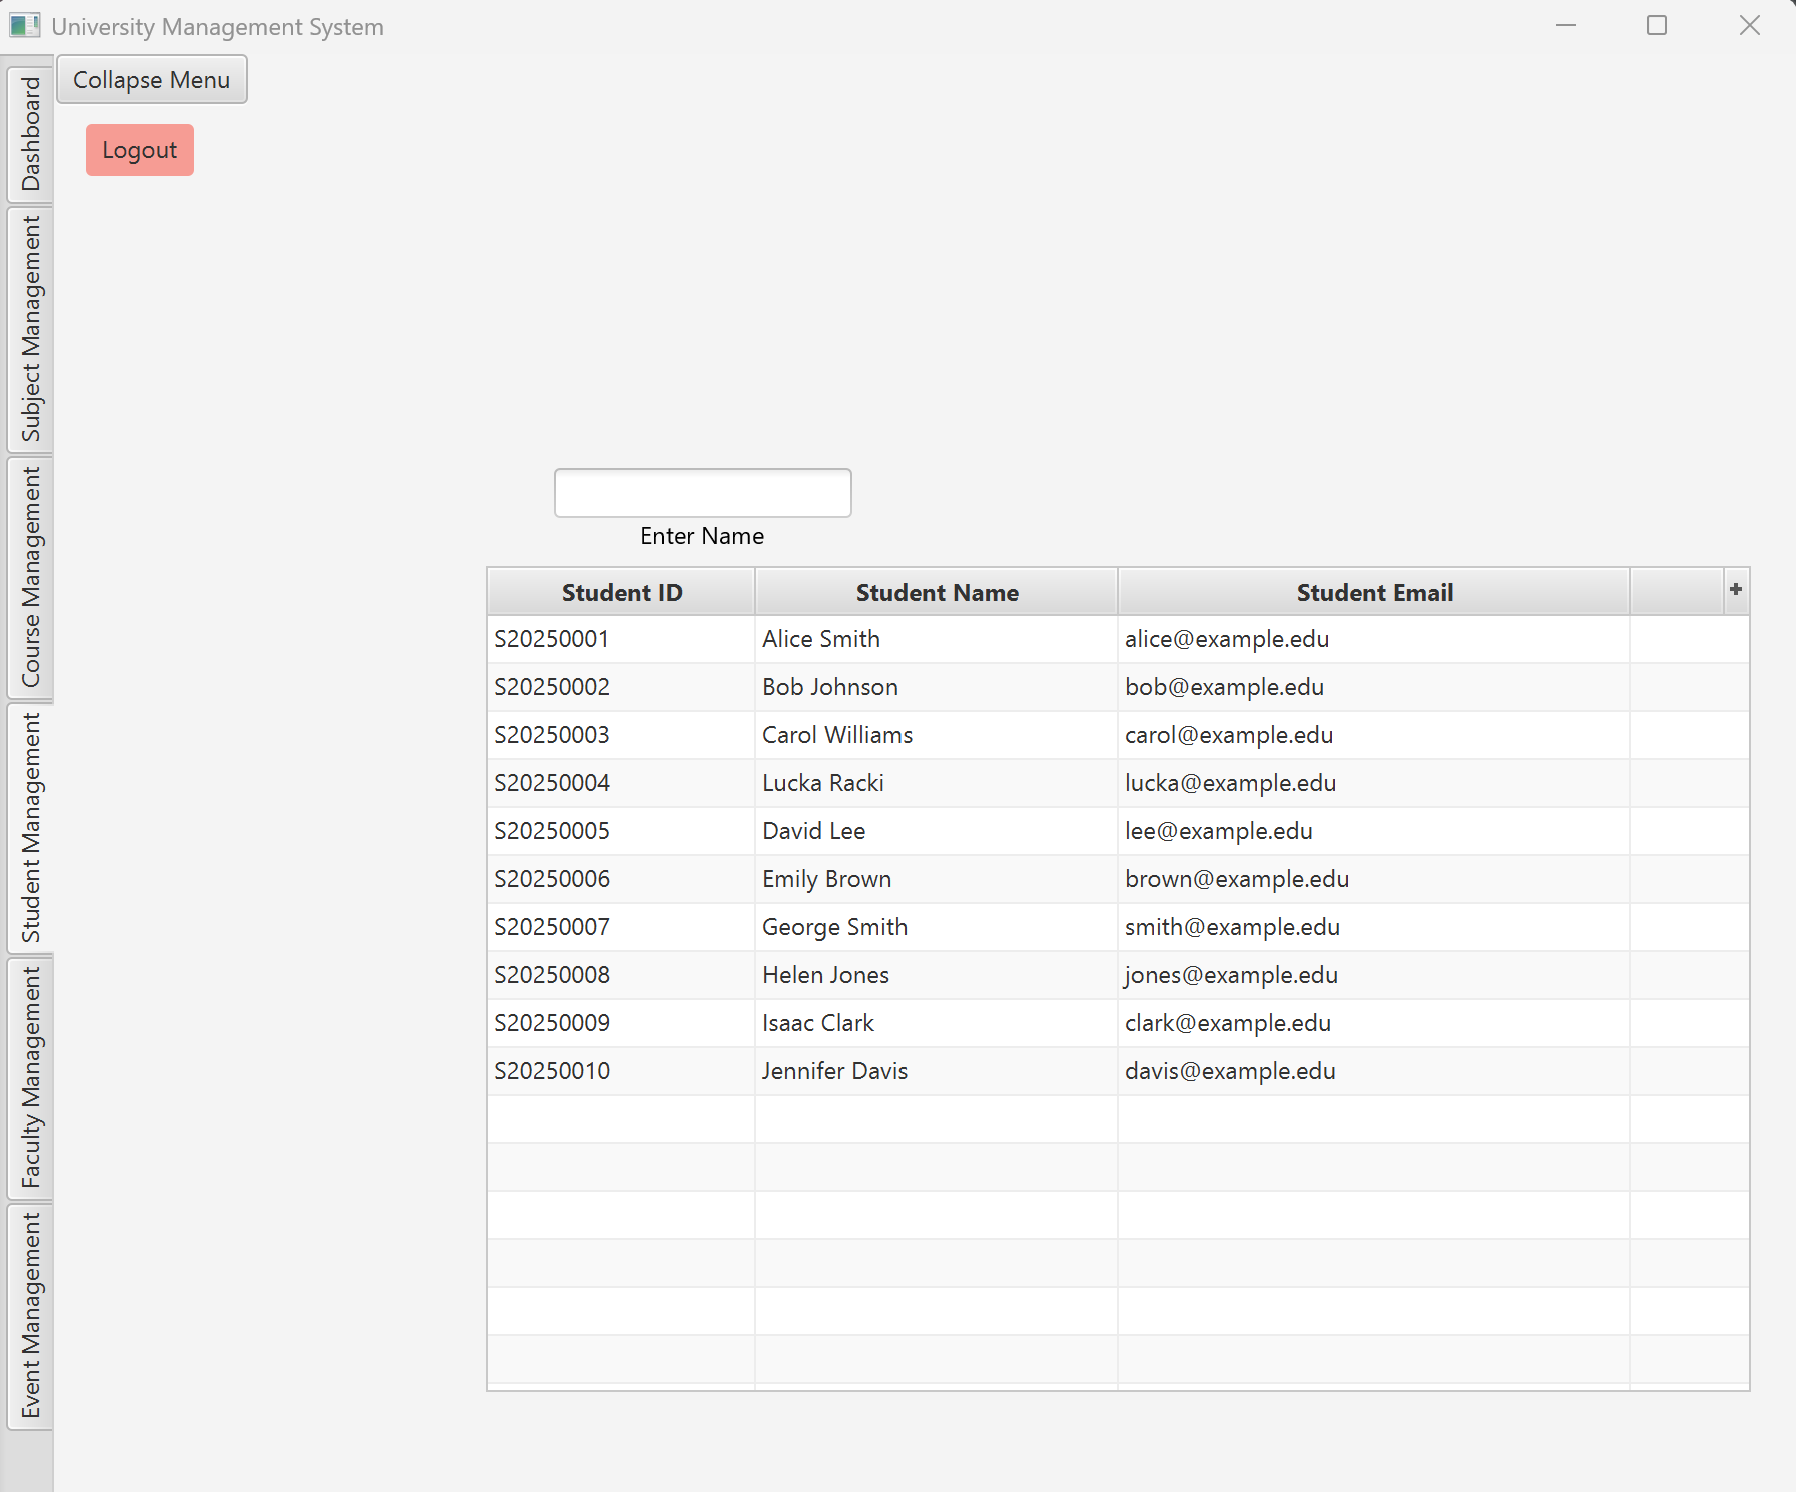
\includegraphics[width=0.7\linewidth]{figures/Student_Management.png}
        \caption{Administrator Login - Student Management Tab}
        \label{fig:example6}
        \FloatBarrier
\end{figure}


The Student Management tab also provides the capability to delete a student. However, this process requires that the administrator selects a student by double-clicking. This allows for a pop-up to occur proving the option to delete a student. Additionally, it provides their student information for the administrator privileges only. Refer to \autoref{fig:example7}.

\begin{figure}[ht!]
    \centering
        \centering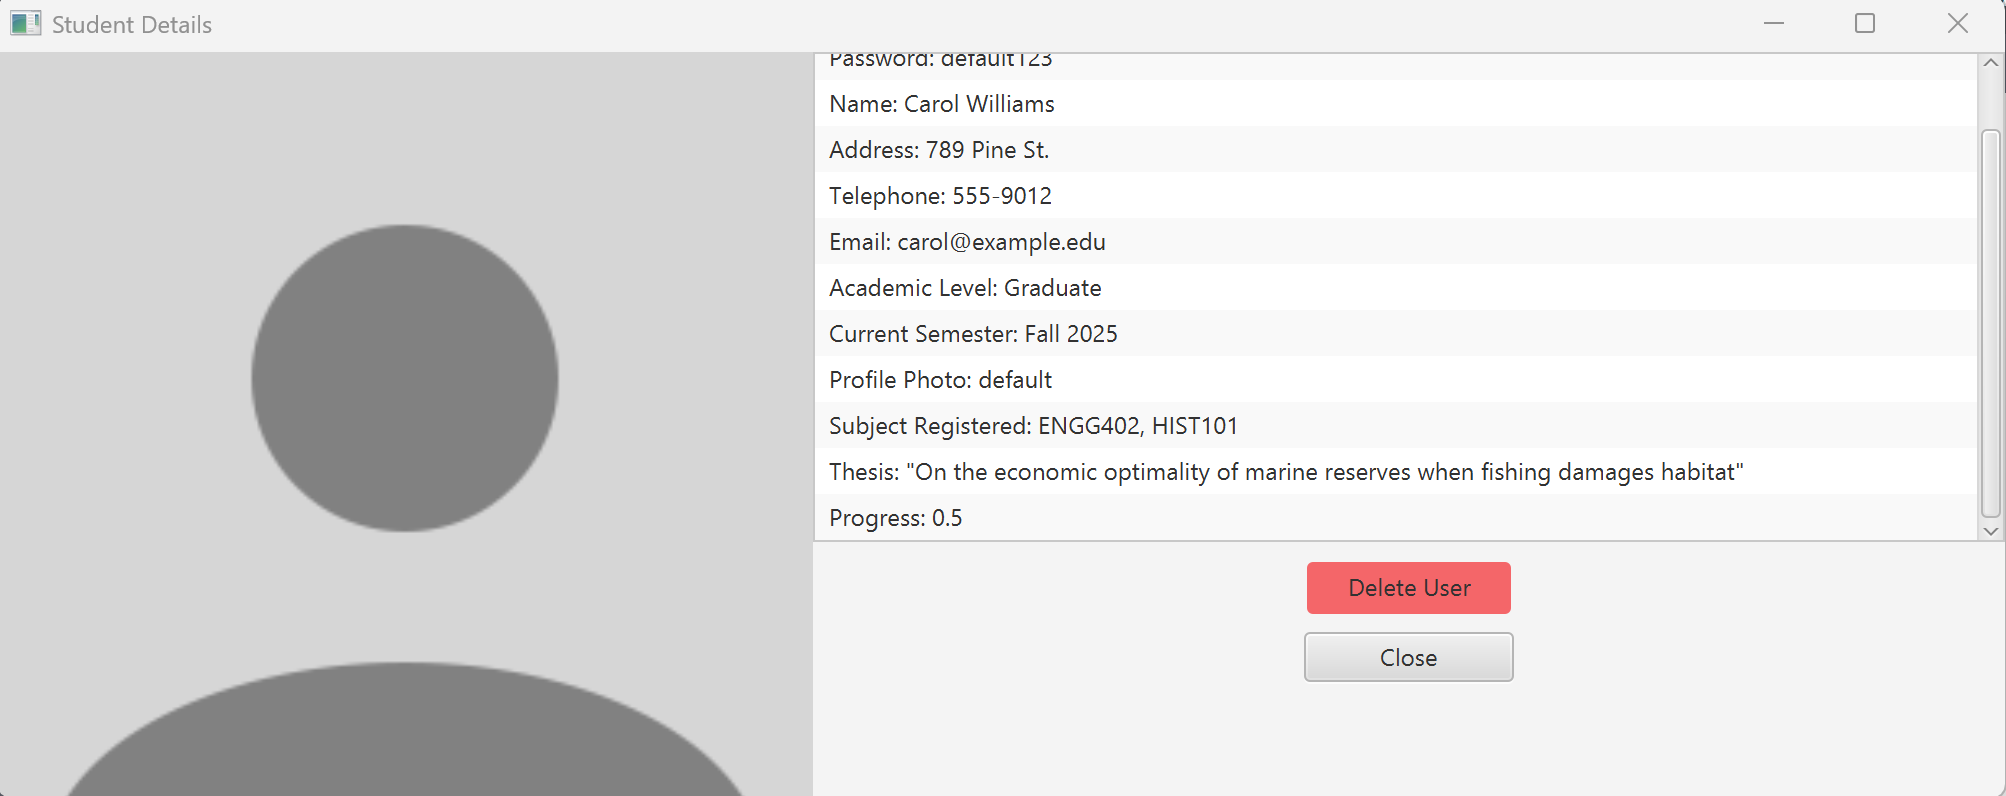
\includegraphics[width=1\linewidth]{figures/Student_Management_Delete.png}
        \caption{Administrator Login - Student Management Tab}
        \label{fig:example7}  
\end{figure}

\newpage
\subsection{Course Management}

The Course Management tab allows the administrator to add and delete courses for the University. Similar to the student management in order to add a course the administrator must utilize the input field box and enter the correct information. For example entering the correct, Course Name, Subject Code, Section Number, Capacity, Lecture Time. Final Exam Date, Location and Teacher. Once all these information have been added it will update in the table showcasing that it was a success.

Deleting a course requires the administrator to complete the following steps:
\begin{enumerate}
    \item Select designated course for deletion
    \item Press the delete course button
    \item Check if it is removed from thr excel data warehouse
\end{enumerate}

Note, that deleting a course is permanent and will require the user to input the same information again if it is deleted.

\begin{figure}[h]
    \centering
        \centering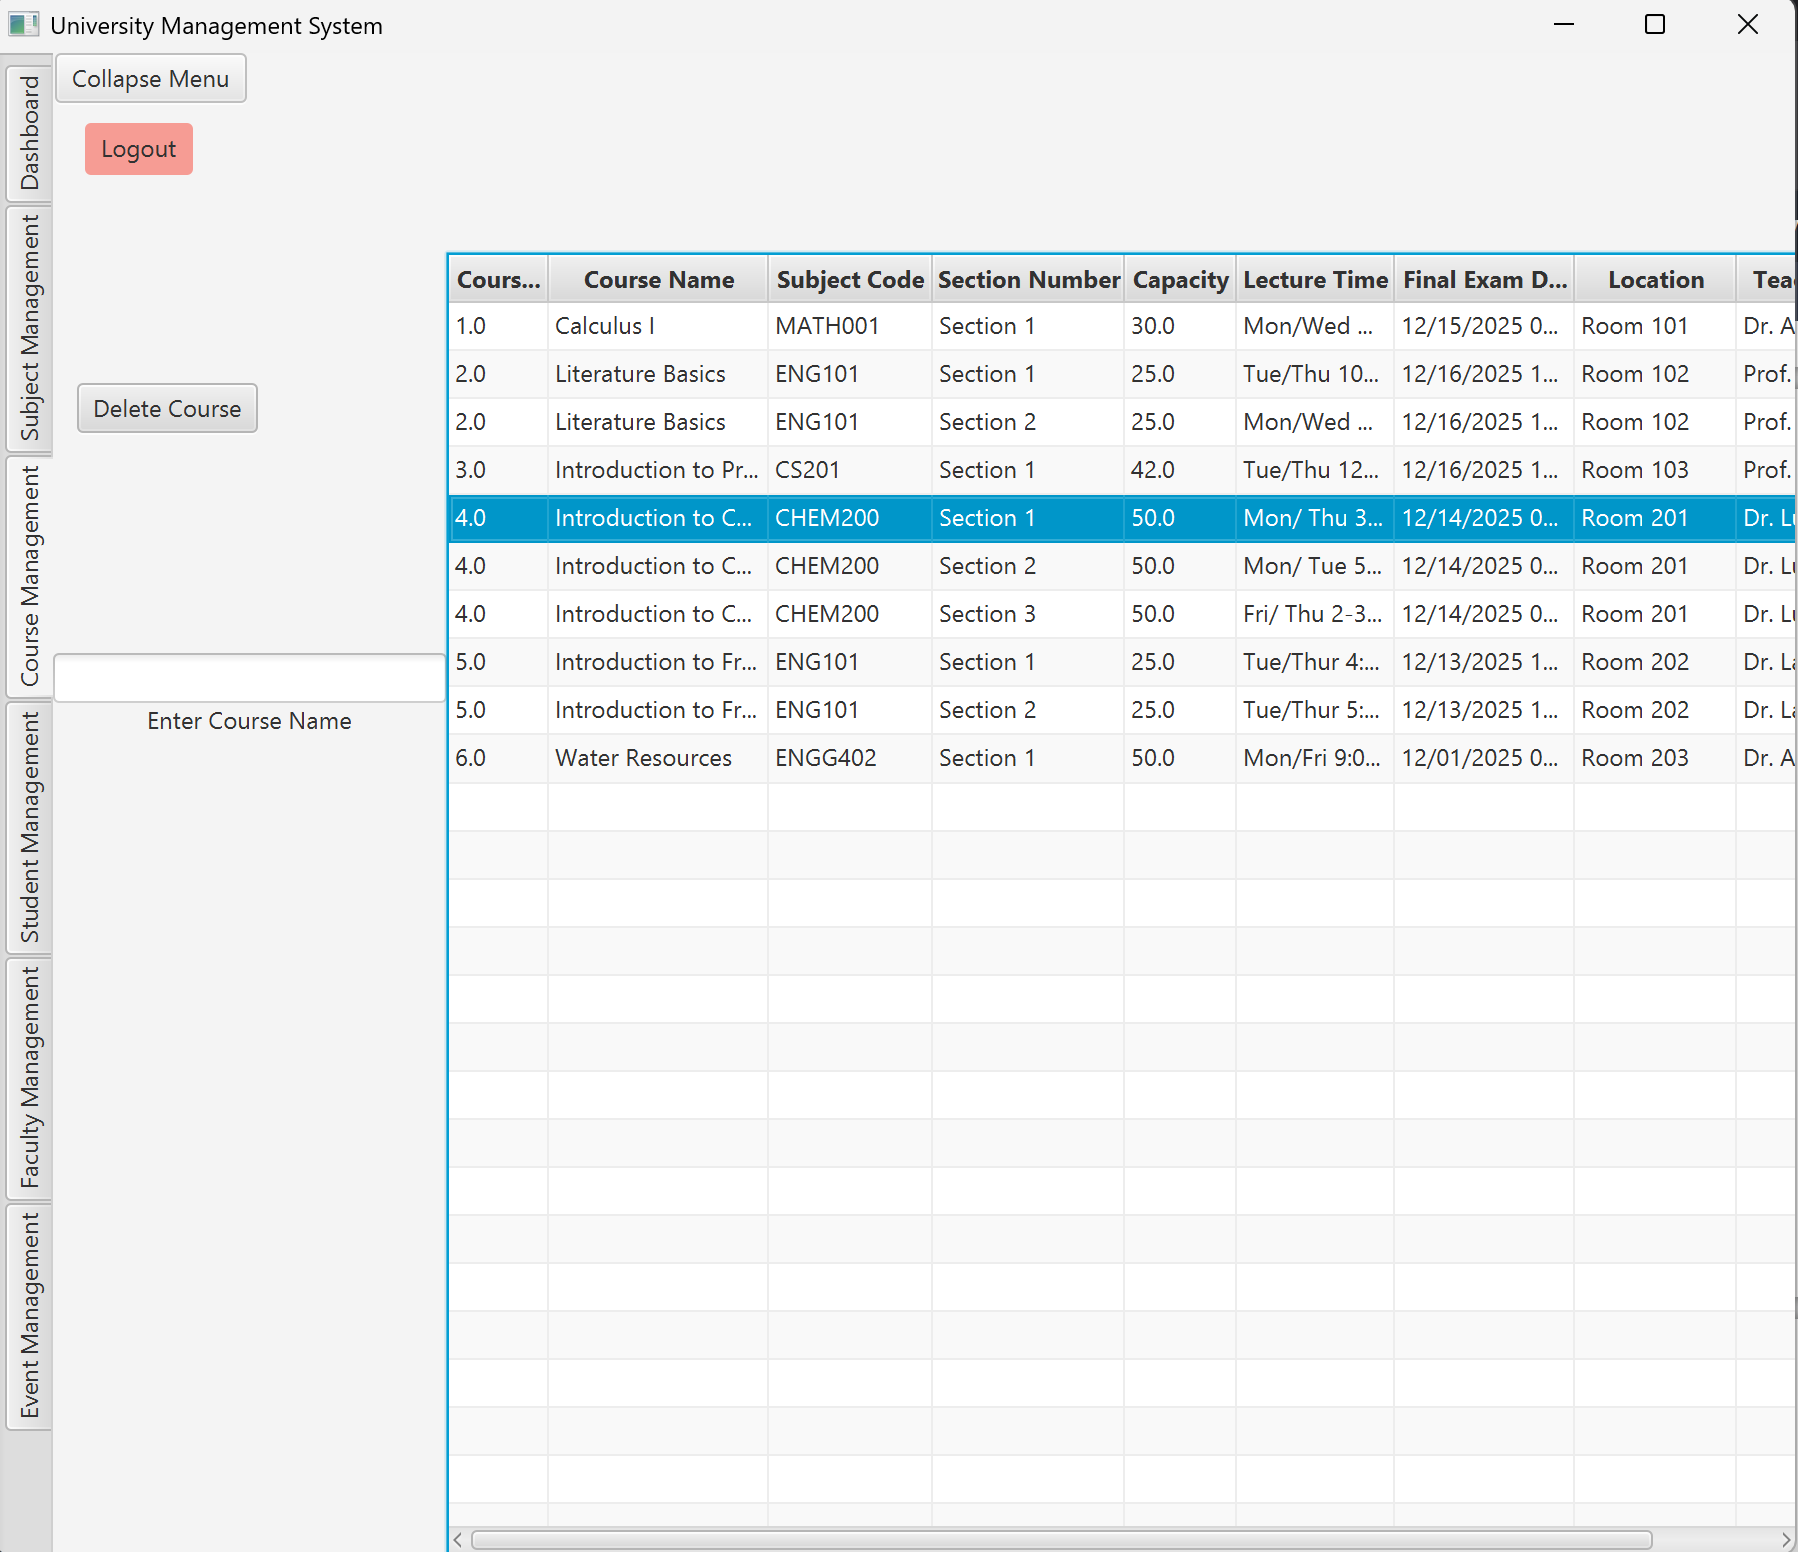
\includegraphics[width=1\linewidth]{figures/Course_Management.png}
        \caption{Administrator Login - Course Management Tab}
        % \label{fig:example11}  
\end{figure}


\subsection{Faculty Management}

The faculty management tab with the administrator login provides the capability to delete and add faculty members (see \autoref{fig:example9}). However, this requires that the course available exist from the course management tab, otherwise selecting the course offered is not possible. In order for an administrator to add a faculty member they must following these steps.

\begin{enumerate}
    \item Select the text box and add the name of the Faculty member
    \item Select the type of degree that they possess, assuming it is either Master's or Ph.D.
    \item Enter their Research interest
    \item Enter their Office Location
    \item Select the Course Offered drop down, assuming it is already included within the course management tab
    \item Press "Add Faculty" button, it will add the Faculty member in the data archive excel file
    \item Observe the added faculty member the in the provided table to the right.
\end{enumerate}


\begin{figure}[ht]
    \centering
        \centering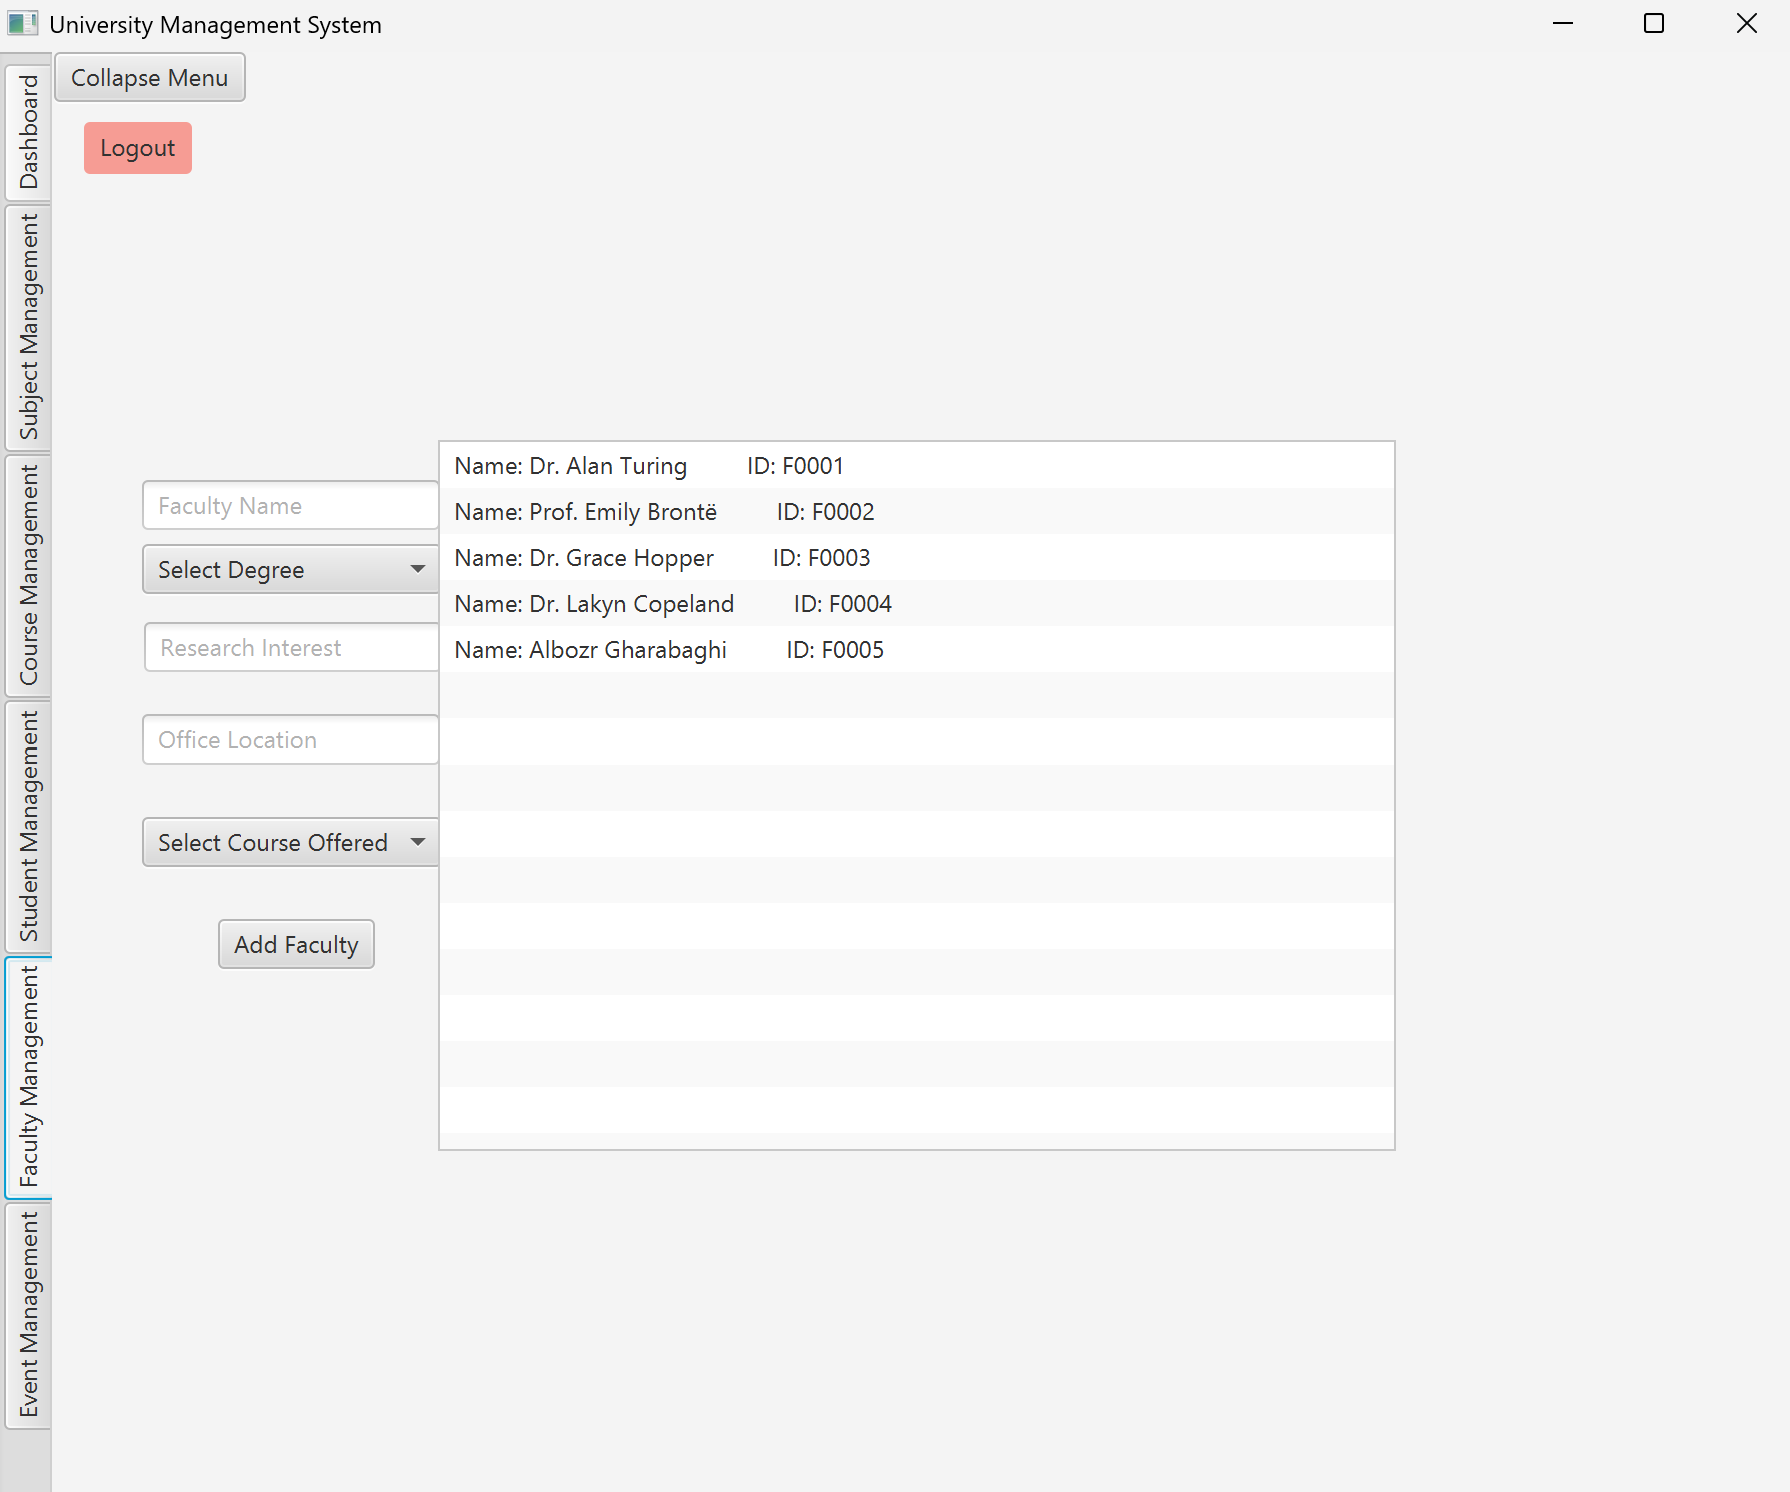
\includegraphics[width=1\linewidth]{figures/Faculty_Management.png}
        \caption{Administrator Login - Faculty Management Tab}
        \label{fig:example9}  
\end{figure}


\newpage
\subsection{Event Management}
The event management tab, focuses on adding events to the calendar that would be relevant to the overall University. This is placed allowing for both faculty and students to be notified on events. Administrators are the only users capable of adding events that remain relevant to the entire University (see \autoref{example10}). The process for adding an event is as follows:
\begin{enumerate}
    \item Enter the Event Date or click the calendar button to auto-select targeted date
    \item Enter the Event Name
    \item Enter the location
    \item Drag the total potential capacity, usually given within the budget or safety protocol
    \item Drag the cost, notice that the it snaps to the closest value of plus minus 0.25, 0.5, 0.75, 1.0
    \item Drag the time it would take for the event, notice it snaps to the closest value rounded by a quarter
    \item Add the event, this should be place in the calendar depending on the selected date.
    
\end{enumerate}

\begin{figure}[ht]
    \centering
        \centering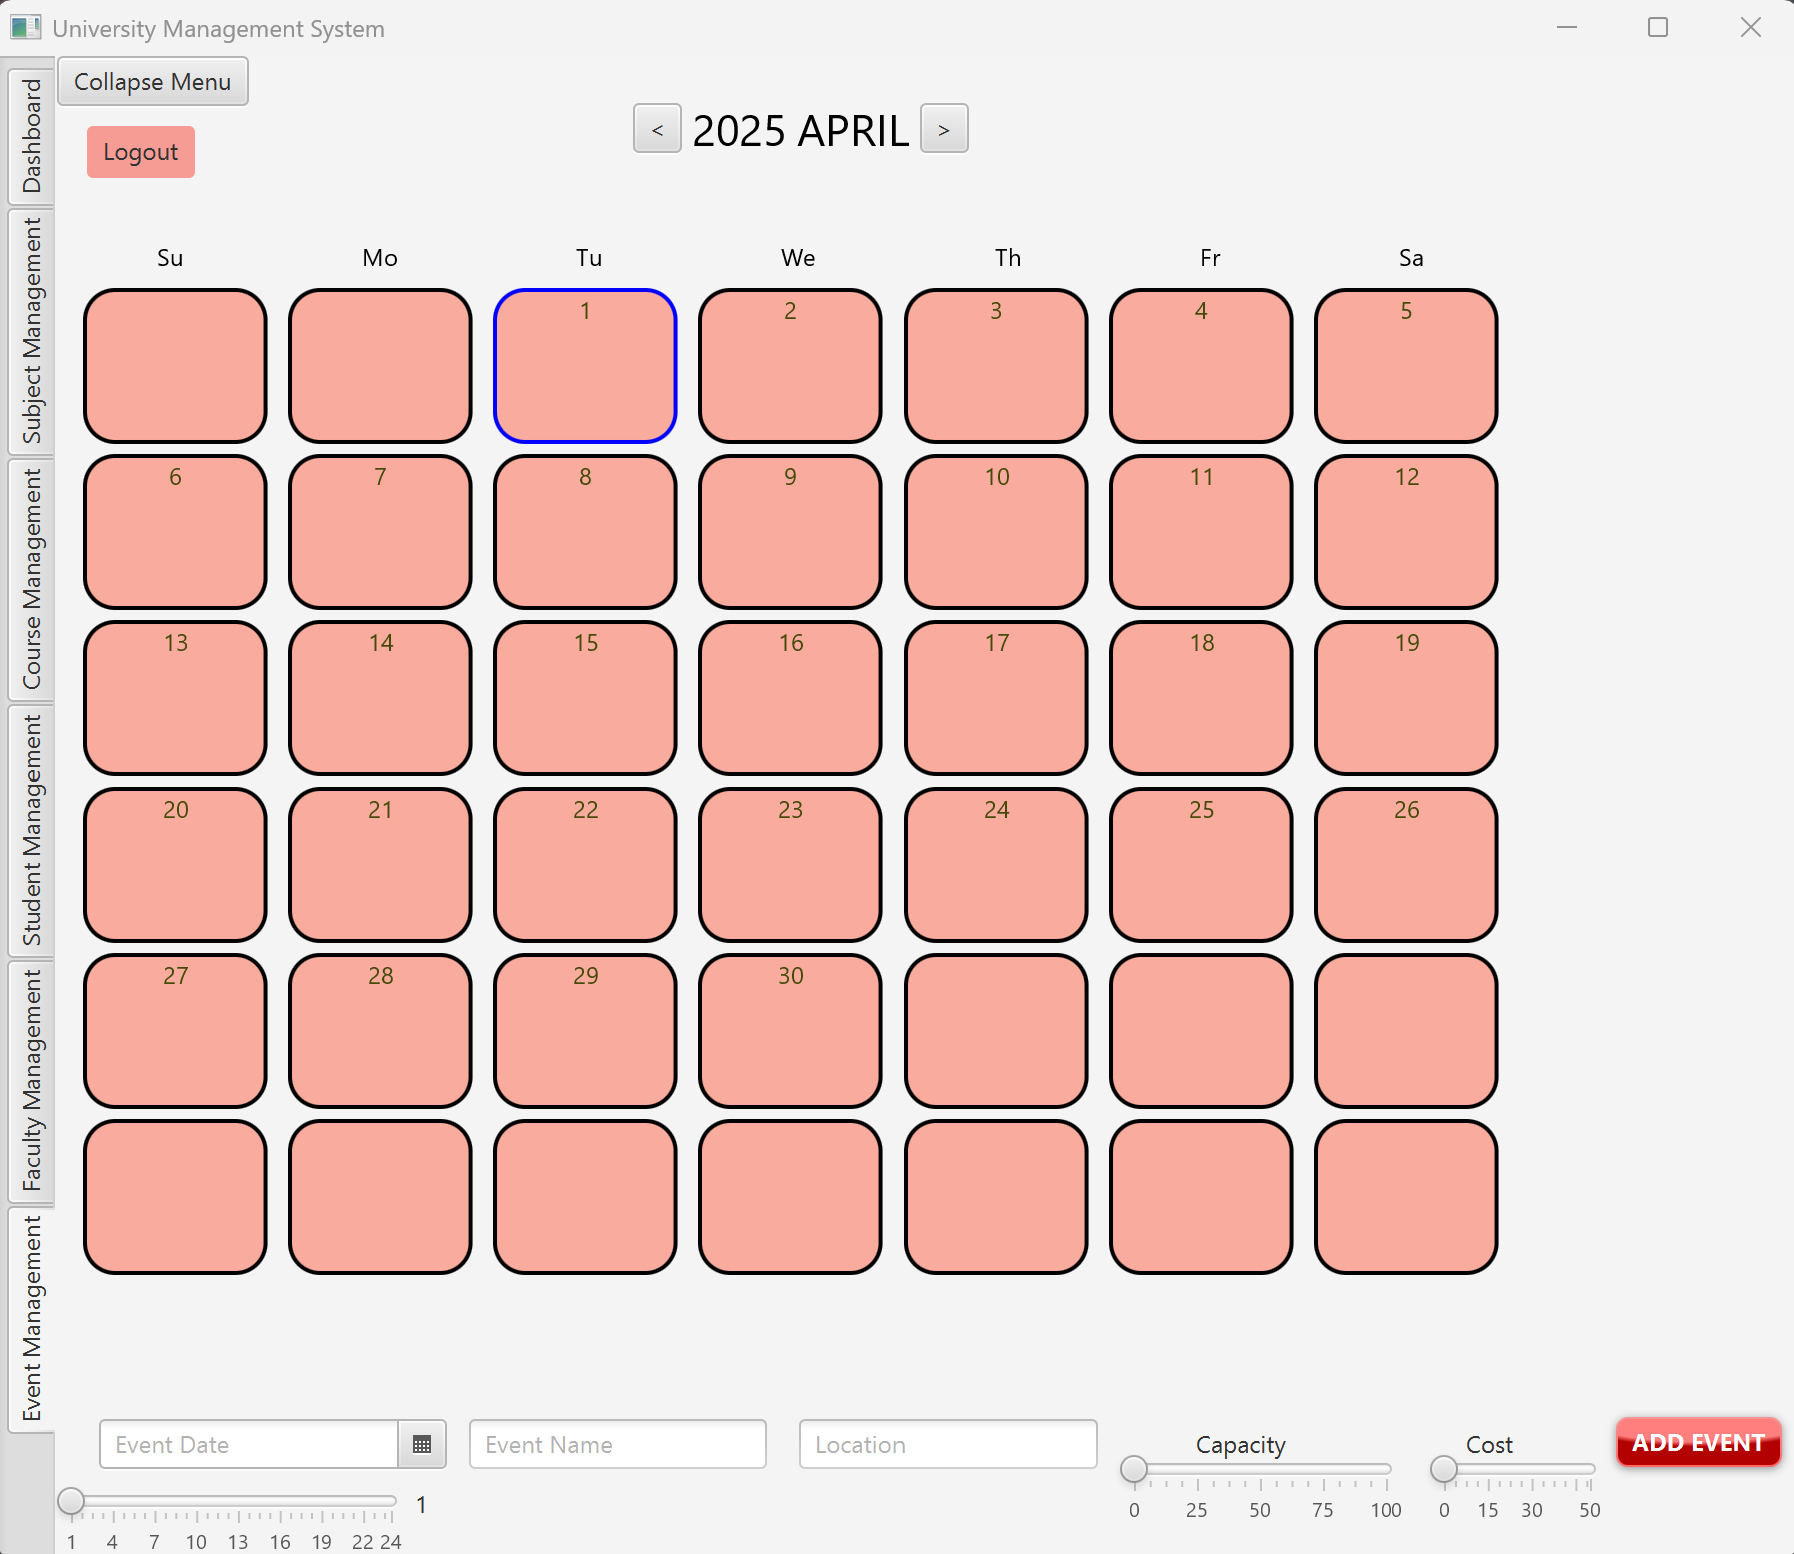
\includegraphics[width=1\linewidth]{figures/Event_Management.png}
        \caption{Administrator Login - Event Management Tab}
        \label{fig:example10}  
\end{figure}